\documentclass[12pt]{article}

%packages
%\usepackage{latexsym}
\usepackage{graphicx}
\usepackage{wrapfig}
\usepackage{color}
\usepackage{amsmath}
%\usepackage{dsfont}
\usepackage{placeins}
\usepackage{amssymb}
\usepackage{skull}
\usepackage{soul}
%\usepackage{hyperref}
%\usepackage{fancyhdr}

%\fancyhf{} % clear all header and footers
%\renewcommand{\headrulewidth}{0pt} % remove the header rule
%\fancyfoot[LE, LO]{\thepage}


%\usepackage{pstricks,pst-node,pst-tree}

%\usepackage{algpseudocode}
%\usepackage{amsthm}
%\usepackage{hyperref}
%\usepackage{mathrsfs}
%\usepackage{amsfonts}
%\usepackage{bbding}
%\usepackage{listings}
%\usepackage{appendix}
\usepackage[margin=1in]{geometry}
%\geometry{papersize={8.5in,11in},total={6.5in,9in}}
%\usepackage{cancel}
%\usepackage{algorithmic, algorithm}

\newcommand{\qu}[1]{``#1''}
\newcommand{\spc}[1]{\\ \vspace{#1cm}}

\newcounter{probnum}
\setcounter{probnum}{1}
\newcounter{numpts}
\setcounter{numpts}{0}

%create definition to allow local margin changes
\def\changemargin#1#2{\list{}{\rightmargin#2\leftmargin#1}\item[]}
\let\endchangemargin=\endlist 

%allow equations to span multiple pages
\allowdisplaybreaks

%define colors and color typesetting conveniences
\definecolor{gray}{rgb}{0.5,0.5,0.5}
\definecolor{black}{rgb}{0,0,0}
\definecolor{white}{rgb}{1,1,1}
\definecolor{blue}{rgb}{0.5,0.5,1}
\newcommand{\inblue}[1]{\color{blue}#1 \color{black}}
\definecolor{green}{rgb}{0.133,0.545,0.133}
\newcommand{\ingreen}[1]{\color{green}#1 \color{black}}
\definecolor{yellow}{rgb}{1,0.549,0}
\newcommand{\inyellow}[1]{\color{yellow}#1 \color{black}}
\definecolor{red}{rgb}{1,0.133,0.133}
\newcommand{\inred}[1]{\color{red}#1 \color{black}}
\definecolor{purple}{rgb}{0.58,0,0.827}
\newcommand{\inpurple}[1]{\color{purple}#1 \color{black}}
\definecolor{gray}{rgb}{0.5,0.5,0.5}
\newcommand{\ingray}[1]{\color{gray}#1 \color{black}}
\definecolor{backgcode}{rgb}{0.97,0.97,0.8}
\definecolor{Brown}{cmyk}{0,0.81,1,0.60}
\definecolor{OliveGreen}{cmyk}{0.64,0,0.95,0.40}
\definecolor{CadetBlue}{cmyk}{0.62,0.57,0.23,0}

%define new math operators
\DeclareMathOperator*{\argmax}{arg\,max~}
\DeclareMathOperator*{\argmin}{arg\,min~}
\DeclareMathOperator*{\argsup}{arg\,sup~}
\DeclareMathOperator*{\arginf}{arg\,inf~}
\DeclareMathOperator*{\convolution}{\text{\Huge{$\ast$}}}
\newcommand{\infconv}[2]{\convolution^\infty_{#1 = 1} #2}
%true functions

%%%% GENERAL SHORTCUTS

%shortcuts for pure typesetting conveniences
\newcommand{\bv}[1]{\boldsymbol{#1}}

%shortcuts for compound constants
\newcommand{\BetaDistrConst}{\dfrac{\Gamma(\alpha + \beta)}{\Gamma(\alpha)\Gamma(\beta)}}
\newcommand{\NormDistrConst}{\dfrac{1}{\sqrt{2\pi\sigma^2}}}

%shortcuts for conventional symbols
\newcommand{\tsq}{\tau^2}
\newcommand{\tsqh}{\hat{\tau}^2}
\newcommand{\sigsq}{\sigma^2}
\newcommand{\sigsqsq}{\parens{\sigma^2}^2}
\newcommand{\sigsqovern}{\dfrac{\sigsq}{n}}
\newcommand{\tausq}{\tau^2}
\newcommand{\tausqalpha}{\tau^2_\alpha}
\newcommand{\tausqbeta}{\tau^2_\beta}
\newcommand{\tausqsigma}{\tau^2_\sigma}
\newcommand{\betasq}{\beta^2}
\newcommand{\sigsqvec}{\bv{\sigma}^2}
\newcommand{\sigsqhat}{\hat{\sigma}^2}
\newcommand{\sigsqhatmlebayes}{\sigsqhat_{\text{Bayes, MLE}}}
\newcommand{\sigsqhatmle}[1]{\sigsqhat_{#1, \text{MLE}}}
\newcommand{\bSigma}{\bv{\Sigma}}
\newcommand{\bSigmainv}{\bSigma^{-1}}
\newcommand{\thetavec}{\bv{\theta}}
\newcommand{\thetahat}{\hat{\theta}}
\newcommand{\thetahatmle}{\hat{\theta}_{\mathrm{MLE}}}
\newcommand{\thetavechatmle}{\hat{\thetavec}_{\mathrm{MLE}}}
\newcommand{\muhat}{\hat{\mu}}
\newcommand{\musq}{\mu^2}
\newcommand{\muvec}{\bv{\mu}}
\newcommand{\muhatmle}{\muhat_{\text{MLE}}}
\newcommand{\lambdahat}{\hat{\lambda}}
\newcommand{\lambdahatmle}{\lambdahat_{\text{MLE}}}
\newcommand{\etavec}{\bv{\eta}}
\newcommand{\alphavec}{\bv{\alpha}}
\newcommand{\minimaxdec}{\delta^*_{\mathrm{mm}}}
\newcommand{\ybar}{\bar{y}}
\newcommand{\xbar}{\bar{x}}
\newcommand{\Xbar}{\bar{X}}
\newcommand{\iid}{~{\buildrel iid \over \sim}~}
\newcommand{\inddist}{~{\buildrel ind \over \sim}~}
\newcommand{\approxdist}{~{\buildrel approx \over \sim}~}
\newcommand{\equalsindist}{~{\buildrel d \over =}~}
\newcommand{\loglik}[1]{\ell\parens{#1}}
\newcommand{\thetahatkminone}{\thetahat^{(k-1)}}
\newcommand{\thetahatkplusone}{\thetahat^{(k+1)}}
\newcommand{\thetahatk}{\thetahat^{(k)}}
\newcommand{\half}{\frac{1}{2}}
\newcommand{\third}{\frac{1}{3}}
\newcommand{\twothirds}{\frac{2}{3}}
\newcommand{\fourth}{\frac{1}{4}}
\newcommand{\fifth}{\frac{1}{5}}
\newcommand{\sixth}{\frac{1}{6}}

%shortcuts for vector and matrix notation
\newcommand{\A}{\bv{A}}
\newcommand{\At}{\A^T}
\newcommand{\Ainv}{\inverse{\A}}
\newcommand{\B}{\bv{B}}
\newcommand{\K}{\bv{K}}
\newcommand{\Kt}{\K^T}
\newcommand{\Kinv}{\inverse{K}}
\newcommand{\Kinvt}{(\Kinv)^T}
\newcommand{\M}{\bv{M}}
\newcommand{\Bt}{\B^T}
\newcommand{\Q}{\bv{Q}}
\newcommand{\Qt}{\Q^T}
\newcommand{\R}{\bv{R}}
\newcommand{\Rt}{\R^T}
\newcommand{\Z}{\bv{Z}}
\newcommand{\X}{\bv{X}}
\newcommand{\Xsub}{\X_{\text{(sub)}}}
\newcommand{\Xsubadj}{\X_{\text{(sub,adj)}}}
\newcommand{\I}{\bv{I}}
\newcommand{\Y}{\bv{Y}}
\newcommand{\sigsqI}{\sigsq\I}
\renewcommand{\P}{\bv{P}}
\newcommand{\Psub}{\P_{\text{(sub)}}}
\newcommand{\Pt}{\P^T}
\newcommand{\Pii}{P_{ii}}
\newcommand{\Pij}{P_{ij}}
\newcommand{\IminP}{(\I-\P)}
\newcommand{\Xt}{\bv{X}^T}
\newcommand{\XtX}{\Xt\X}
\newcommand{\XtXinv}{\parens{\Xt\X}^{-1}}
\newcommand{\XtXinvXt}{\XtXinv\Xt}
\newcommand{\XXtXinvXt}{\X\XtXinvXt}
\newcommand{\x}{\bv{x}}
\newcommand{\onevec}{\bv{1}}
\newcommand{\oneton}{1, \ldots, n}
\newcommand{\yoneton}{y_1, \ldots, y_n}
\newcommand{\yonetonorder}{y_{(1)}, \ldots, y_{(n)}}
\newcommand{\Yoneton}{Y_1, \ldots, Y_n}
\newcommand{\iinoneton}{i \in \braces{\oneton}}
\newcommand{\onetom}{1, \ldots, m}
\newcommand{\jinonetom}{j \in \braces{\onetom}}
\newcommand{\xoneton}{x_1, \ldots, x_n}
\newcommand{\Xoneton}{X_1, \ldots, X_n}
\newcommand{\xt}{\x^T}
\newcommand{\y}{\bv{y}}
\newcommand{\yt}{\y^T}
\renewcommand{\c}{\bv{c}}
\newcommand{\ct}{\c^T}
\newcommand{\tstar}{\bv{t}^*}
\renewcommand{\u}{\bv{u}}
\renewcommand{\v}{\bv{v}}
\renewcommand{\a}{\bv{a}}
\newcommand{\s}{\bv{s}}
\newcommand{\yadj}{\y_{\text{(adj)}}}
\newcommand{\xjadj}{\x_{j\text{(adj)}}}
\newcommand{\xjadjM}{\x_{j \perp M}}
\newcommand{\yhat}{\hat{\y}}
\newcommand{\yhatsub}{\yhat_{\text{(sub)}}}
\newcommand{\yhatstar}{\yhat^*}
\newcommand{\yhatstarnew}{\yhatstar_{\text{new}}}
\newcommand{\z}{\bv{z}}
\newcommand{\zt}{\z^T}
\newcommand{\bb}{\bv{b}}
\newcommand{\bbt}{\bb^T}
\newcommand{\bbeta}{\bv{\beta}}
\newcommand{\beps}{\bv{\epsilon}}
\newcommand{\bepst}{\beps^T}
\newcommand{\e}{\bv{e}}
\newcommand{\Mofy}{\M(\y)}
\newcommand{\KofAlpha}{K(\alpha)}
\newcommand{\ellset}{\mathcal{L}}
\newcommand{\oneminalph}{1-\alpha}
\newcommand{\SSE}{\text{SSE}}
\newcommand{\SSEsub}{\text{SSE}_{\text{(sub)}}}
\newcommand{\MSE}{\text{MSE}}
\newcommand{\RMSE}{\text{RMSE}}
\newcommand{\SSR}{\text{SSR}}
\newcommand{\SST}{\text{SST}}
\newcommand{\JSest}{\delta_{\text{JS}}(\x)}
\newcommand{\Bayesest}{\delta_{\text{Bayes}}(\x)}
\newcommand{\EmpBayesest}{\delta_{\text{EmpBayes}}(\x)}
\newcommand{\BLUPest}{\delta_{\text{BLUP}}}
\newcommand{\MLEest}[1]{\hat{#1}_{\text{MLE}}}

%shortcuts for Linear Algebra stuff (i.e. vectors and matrices)
\newcommand{\twovec}[2]{\bracks{\begin{array}{c} #1 \\ #2 \end{array}}}
\newcommand{\threevec}[3]{\bracks{\begin{array}{c} #1 \\ #2 \\ #3 \end{array}}}
\newcommand{\fivevec}[5]{\bracks{\begin{array}{c} #1 \\ #2 \\ #3 \\ #4 \\ #5 \end{array}}}
\newcommand{\twobytwomat}[4]{\bracks{\begin{array}{cc} #1 & #2 \\ #3 & #4 \end{array}}}
\newcommand{\threebytwomat}[6]{\bracks{\begin{array}{cc} #1 & #2 \\ #3 & #4 \\ #5 & #6 \end{array}}}

%shortcuts for conventional compound symbols
\newcommand{\thetainthetas}{\theta \in \Theta}
\newcommand{\reals}{\mathbb{R}}
\newcommand{\complexes}{\mathbb{C}}
\newcommand{\rationals}{\mathbb{Q}}
\newcommand{\integers}{\mathbb{Z}}
\newcommand{\naturals}{\mathbb{N}}
\newcommand{\forallninN}{~~\forall n \in \naturals}
\newcommand{\forallxinN}[1]{~~\forall #1 \in \reals}
\newcommand{\matrixdims}[2]{\in \reals^{\,#1 \times #2}}
\newcommand{\inRn}[1]{\in \reals^{\,#1}}
\newcommand{\mathimplies}{\quad\Rightarrow\quad}
\newcommand{\mathlogicequiv}{\quad\Leftrightarrow\quad}
\newcommand{\eqncomment}[1]{\quad \text{(#1)}}
\newcommand{\limitn}{\lim_{n \rightarrow \infty}}
\newcommand{\limitN}{\lim_{N \rightarrow \infty}}
\newcommand{\limitd}{\lim_{d \rightarrow \infty}}
\newcommand{\limitt}{\lim_{t \rightarrow \infty}}
\newcommand{\limitsupn}{\limsup_{n \rightarrow \infty}~}
\newcommand{\limitinfn}{\liminf_{n \rightarrow \infty}~}
\newcommand{\limitk}{\lim_{k \rightarrow \infty}}
\newcommand{\limsupn}{\limsup_{n \rightarrow \infty}}
\newcommand{\limsupk}{\limsup_{k \rightarrow \infty}}
\newcommand{\floor}[1]{\left\lfloor #1 \right\rfloor}
\newcommand{\ceil}[1]{\left\lceil #1 \right\rceil}

%shortcuts for environments
\newcommand{\beqn}{\vspace{-0.25cm}\begin{eqnarray*}}
\newcommand{\eeqn}{\end{eqnarray*}}
\newcommand{\bneqn}{\vspace{-0.25cm}\begin{eqnarray}}
\newcommand{\eneqn}{\end{eqnarray}}
\newcommand{\benum}{\begin{enumerate}}
\newcommand{\eenum}{\end{enumerate}}

%shortcuts for mini environments
\newcommand{\parens}[1]{\left(#1\right)}
\newcommand{\squared}[1]{\parens{#1}^2}
\newcommand{\tothepow}[2]{\parens{#1}^{#2}}
\newcommand{\prob}[1]{\mathbb{P}\parens{#1}}
\newcommand{\littleo}[1]{o\parens{#1}}
\newcommand{\bigo}[1]{O\parens{#1}}
\newcommand{\Lp}[1]{\mathbb{L}^{#1}}
\renewcommand{\arcsin}[1]{\text{arcsin}\parens{#1}}
\newcommand{\prodonen}[2]{\bracks{\prod_{#1=1}^n #2}}
\newcommand{\mysum}[4]{\sum_{#1=#2}^{#3} #4}
\newcommand{\sumonen}[2]{\sum_{#1=1}^n #2}
\newcommand{\infsum}[2]{\sum_{#1=1}^\infty #2}
\newcommand{\infprod}[2]{\prod_{#1=1}^\infty #2}
\newcommand{\infunion}[2]{\bigcup_{#1=1}^\infty #2}
\newcommand{\infinter}[2]{\bigcap_{#1=1}^\infty #2}
\newcommand{\infintegral}[2]{\int^\infty_{-\infty} #2 ~\text{d}#1}
\newcommand{\supthetas}[1]{\sup_{\thetainthetas}\braces{#1}}
\newcommand{\bracks}[1]{\left[#1\right]}
\newcommand{\braces}[1]{\left\{#1\right\}}
\newcommand{\set}[1]{\left\{#1\right\}}
\newcommand{\abss}[1]{\left|#1\right|}
\newcommand{\norm}[1]{\left|\left|#1\right|\right|}
\newcommand{\normsq}[1]{\norm{#1}^2}
\newcommand{\inverse}[1]{\parens{#1}^{-1}}
\newcommand{\rowof}[2]{\parens{#1}_{#2\cdot}}

%shortcuts for functionals
\newcommand{\realcomp}[1]{\text{Re}\bracks{#1}}
\newcommand{\imagcomp}[1]{\text{Im}\bracks{#1}}
\newcommand{\range}[1]{\text{range}\bracks{#1}}
\newcommand{\colsp}[1]{\text{colsp}\bracks{#1}}
\newcommand{\rowsp}[1]{\text{rowsp}\bracks{#1}}
\newcommand{\tr}[1]{\text{tr}\bracks{#1}}
\newcommand{\rank}[1]{\text{rank}\bracks{#1}}
\newcommand{\proj}[2]{\text{Proj}_{#1}\bracks{#2}}
\newcommand{\projcolspX}[1]{\text{Proj}_{\colsp{\X}}\bracks{#1}}
\newcommand{\median}[1]{\text{median}\bracks{#1}}
\newcommand{\mean}[1]{\text{mean}\bracks{#1}}
\newcommand{\dime}[1]{\text{dim}\bracks{#1}}
\renewcommand{\det}[1]{\text{det}\bracks{#1}}
\newcommand{\expe}[1]{\mathbb{E}\bracks{#1}}
\newcommand{\expeabs}[1]{\expe{\abss{#1}}}
\newcommand{\expesub}[2]{\mathbb{E}_{#1}\bracks{#2}}
\newcommand{\indic}[1]{\mathds{1}_{#1}}
\newcommand{\var}[1]{\mathbb{V}\text{ar}\bracks{#1}}
\newcommand{\sd}[1]{\mathbb{S}\text{D}\bracks{#1}}
\newcommand{\cov}[2]{\text{Cov}\bracks{#1, #2}}
\newcommand{\corr}[2]{\text{Corr}\bracks{#1, #2}}
\newcommand{\se}[1]{\text{SE}\bracks{#1}}
\newcommand{\seest}[1]{\hat{\text{SE}}\bracks{#1}}
\newcommand{\bias}[1]{\text{Bias}\bracks{#1}}
\newcommand{\partialop}[2]{\dfrac{\partial}{\partial #1}\bracks{#2}}
\newcommand{\secpartialop}[2]{\dfrac{\partial^2}{\partial #1^2}\bracks{#2}}
\newcommand{\mixpartialop}[3]{\dfrac{\partial^2}{\partial #1 \partial #2}\bracks{#3}}

%shortcuts for functions
\renewcommand{\exp}[1]{\mathrm{exp}\parens{#1}}
\renewcommand{\cos}[1]{\text{cos}\parens{#1}}
\renewcommand{\sin}[1]{\text{sin}\parens{#1}}
\newcommand{\sign}[1]{\text{sign}\parens{#1}}
\newcommand{\are}[1]{\mathrm{ARE}\parens{#1}}
\newcommand{\natlog}[1]{\ln\parens{#1}}
\newcommand{\oneover}[1]{\frac{1}{#1}}
\newcommand{\overtwo}[1]{\frac{#1}{2}}
\newcommand{\overn}[1]{\frac{#1}{n}}
\newcommand{\oneoversqrt}[1]{\oneover{\sqrt{#1}}}
\newcommand{\sqd}[1]{\parens{#1}^2}
\newcommand{\loss}[1]{\ell\parens{\theta, #1}}
\newcommand{\losstwo}[2]{\ell\parens{#1, #2}}
\newcommand{\cf}{\phi(t)}

%English language specific shortcuts
\newcommand{\ie}{\textit{i.e.} }
\newcommand{\AKA}{\textit{AKA} }
\renewcommand{\iff}{\textit{iff}}
\newcommand{\eg}{\textit{e.g.} }
\renewcommand{\st}{\textit{s.t.} }
\newcommand{\wrt}{\textit{w.r.t.} }
\newcommand{\mathst}{~~\text{\st}~~}
\newcommand{\mathand}{~~\text{and}~~}
\newcommand{\ala}{\textit{a la} }
\newcommand{\ppp}{posterior predictive p-value}
\newcommand{\dd}{dataset-to-dataset}

%shortcuts for distribution titles
\newcommand{\logistic}[2]{\mathrm{Logistic}\parens{#1,\,#2}}
\newcommand{\bernoulli}[1]{\mathrm{Bernoulli}\parens{#1}}
\newcommand{\betanot}[2]{\mathrm{Beta}\parens{#1,\,#2}}
\newcommand{\stdbetanot}{\betanot{\alpha}{\beta}}
\newcommand{\multnormnot}[3]{\mathcal{N}_{#1}\parens{#2,\,#3}}
\newcommand{\normnot}[2]{\mathcal{N}\parens{#1,\,#2}}
\newcommand{\classicnormnot}{\normnot{\mu}{\sigsq}}
\newcommand{\stdnormnot}{\normnot{0}{1}}
\newcommand{\uniform}[2]{\mathrm{U}\parens{#1,\,#2}}
\newcommand{\stduniform}{\uniform{0}{1}}
\newcommand{\exponential}[1]{\mathrm{Exp}\parens{#1}}
\newcommand{\gammadist}[2]{\mathrm{Gamma}\parens{#1, #2}}
\newcommand{\poisson}[1]{\mathrm{Poisson}\parens{#1}}
\newcommand{\binomial}[2]{\mathrm{Binomial}\parens{#1,\,#2}}
\newcommand{\rayleigh}[1]{\mathrm{Rayleigh}\parens{#1}}
\newcommand{\multinomial}[2]{\mathrm{Multinomial}\parens{#1,\,#2}}
\newcommand{\gammanot}[2]{\mathrm{Gamma}\parens{#1,\,#2}}
\newcommand{\cauchynot}[2]{\text{Cauchy}\parens{#1,\,#2}}
\newcommand{\invchisqnot}[1]{\text{Inv}\chisq{#1}}
\newcommand{\invscaledchisqnot}[2]{\text{ScaledInv}\ncchisq{#1}{#2}}
\newcommand{\invgammanot}[2]{\text{InvGamma}\parens{#1,\,#2}}
\newcommand{\chisq}[1]{\chi^2_{#1}}
\newcommand{\ncchisq}[2]{\chi^2_{#1}\parens{#2}}
\newcommand{\ncF}[3]{F_{#1,#2}\parens{#3}}

%shortcuts for PDF's of common distributions
\newcommand{\logisticpdf}[3]{\oneover{#3}\dfrac{\exp{-\dfrac{#1 - #2}{#3}}}{\parens{1+\exp{-\dfrac{#1 - #2}{#3}}}^2}}
\newcommand{\betapdf}[3]{\dfrac{\Gamma(#2 + #3)}{\Gamma(#2)\Gamma(#3)}#1^{#2-1} (1-#1)^{#3-1}}
\newcommand{\normpdf}[3]{\frac{1}{\sqrt{2\pi#3}}\exp{-\frac{1}{2#3}(#1 - #2)^2}}
\newcommand{\normpdfvarone}[2]{\dfrac{1}{\sqrt{2\pi}}e^{-\half(#1 - #2)^2}}
\newcommand{\chisqpdf}[2]{\dfrac{1}{2^{#2/2}\Gamma(#2/2)}\; {#1}^{#2/2-1} e^{-#1/2}}
\newcommand{\invchisqpdf}[2]{\dfrac{2^{-\overtwo{#1}}}{\Gamma(#2/2)}\,{#1}^{-\overtwo{#2}-1}  e^{-\oneover{2 #1}}}
\newcommand{\uniformdiscrete}[1]{\mathrm{Uniform}\parens{\braces{#1}}}
\newcommand{\exponentialpdf}[2]{#2\exp{-#2#1}}
\newcommand{\poissonpdf}[2]{\dfrac{e^{-#1} #1^{#2}}{#2!}}
\newcommand{\binomialpdf}[3]{\binom{#2}{#1}#3^{#1}(1-#3)^{#2-#1}}
\newcommand{\rayleighpdf}[2]{\dfrac{#1}{#2^2}\exp{-\dfrac{#1^2}{2 #2^2}}}
\newcommand{\gammapdf}[3]{\dfrac{#3^#2}{\Gamma\parens{#2}}#1^{#2-1}\exp{-#3 #1}}
\newcommand{\cauchypdf}[3]{\oneover{\pi} \dfrac{#3}{\parens{#1-#2}^2 + #3^2}}
\newcommand{\Gammaf}[1]{\Gamma\parens{#1}}

%shortcuts for miscellaneous typesetting conveniences
\newcommand{\notesref}[1]{\marginpar{\color{gray}\tt #1\color{black}}}

%%%% DOMAIN-SPECIFIC SHORTCUTS

%Real analysis related shortcuts
\newcommand{\zeroonecl}{\bracks{0,1}}
\newcommand{\forallepsgrzero}{\forall \epsilon > 0~~}
\newcommand{\lessthaneps}{< \epsilon}
\newcommand{\fraccomp}[1]{\text{frac}\bracks{#1}}

%Bayesian related shortcuts
\newcommand{\yrep}{y^{\text{rep}}}
\newcommand{\yrepisq}{(\yrep_i)^2}
\newcommand{\yrepvec}{\bv{y}^{\text{rep}}}


%Probability shortcuts
\newcommand{\SigField}{\mathcal{F}}
\newcommand{\ProbMap}{\mathcal{P}}
\newcommand{\probtrinity}{\parens{\Omega, \SigField, \ProbMap}}
\newcommand{\convp}{~{\buildrel p \over \rightarrow}~}
\newcommand{\convLp}[1]{~{\buildrel \Lp{#1} \over \rightarrow}~}
\newcommand{\nconvp}{~{\buildrel p \over \nrightarrow}~}
\newcommand{\convae}{~{\buildrel a.e. \over \longrightarrow}~}
\newcommand{\convau}{~{\buildrel a.u. \over \longrightarrow}~}
\newcommand{\nconvau}{~{\buildrel a.u. \over \nrightarrow}~}
\newcommand{\nconvae}{~{\buildrel a.e. \over \nrightarrow}~}
\newcommand{\convd}{~{\buildrel \mathcal{D} \over \rightarrow}~}
\newcommand{\nconvd}{~{\buildrel \mathcal{D} \over \nrightarrow}~}
\newcommand{\withprob}{~~\text{w.p.}~~}
\newcommand{\io}{~~\text{i.o.}}

\newcommand{\Acl}{\bar{A}}
\newcommand{\ENcl}{\bar{E}_N}
\newcommand{\diam}[1]{\text{diam}\parens{#1}}

\newcommand{\taua}{\tau_a}

\newcommand{\myint}[4]{\int_{#2}^{#3} #4 \,\text{d}#1}
\newcommand{\laplacet}[1]{\mathscr{L}\bracks{#1}}
\newcommand{\laplaceinvt}[1]{\mathscr{L}^{-1}\bracks{#1}}
\renewcommand{\min}[1]{\text{min}\braces{#1}}

\newcommand{\Vbar}[1]{\bar{V}\parens{#1}}
\newcommand{\expnegrtau}{\exp{-r\tau}}
\newcommand{\cprob}[2]{\prob{#1~|~#2}}

%%% problem typesetting
\newcommand{\problem}{\vspace{0.2cm} \noindent {\large{\textsf{Problem \arabic{probnum}~}}} \addtocounter{probnum}{1}}
%\newcommand{\easyproblem}{\ingreen{\noindent \textsf{Problem \arabic{probnum}~}} \addtocounter{probnum}{1}}
%\newcommand{\intermediateproblem}{\noindent \inyellow{\textsf{Problem \arabic{probnum}~}} \addtocounter{probnum}{1}}
%\newcommand{\hardproblem}{\inred{\noindent \textsf{Problem \arabic{probnum}~}} \addtocounter{probnum}{1}}
%\newcommand{\extracreditproblem}{\noindent \inpurple{\textsf{Problem \arabic{probnum}~}} \addtocounter{probnum}{1}}

\newcommand{\easysubproblem}{\ingreen{\item}}
\newcommand{\intermediatesubproblem}{\inyellow{\item}}
\newcommand{\hardsubproblem}{\inred{\item}}
\newcommand{\extracreditsubproblem}{\inpurple{\item}}
\renewcommand{\labelenumi}{(\alph{enumi})}
%\newcommand{\subquestionwithpoints}[1]{\addtocounter{numpts}{#1} \item \ingray{[#1 pt]}~~} %  / \arabic{numpts} pts
\newcommand{\subquestionwithpoints}[1]{\addtocounter{numpts}{#1} \item \ingray{[#1 pt / \arabic{numpts} pts]}~~}  
\usepackage{textcomp}
\usepackage{tfrupee} 
\pdfmapfile{=tfrupee.map}

\title{Math 241 Fall 2016 \\ Midterm Examination Two}
\author{Professor Adam Kapelner}

\date{November 15, 2016}

\begin{document}
\maketitle

\noindent Full Name \line(1,0){270} ~~~ Section (A or B)~ \line(1,0){30}

\thispagestyle{empty}

\section*{Code of Academic Integrity}

\footnotesize
Since the college is an academic community, its fundamental purpose is the pursuit of knowledge. Essential to the success of this educational mission is a commitment to the principles of academic integrity. Every member of the college community is responsible for upholding the highest standards of honesty at all times. Students, as members of the community, are also responsible for adhering to the principles and spirit of the following Code of Academic Integrity.

Activities that have the effect or intention of interfering with education, pursuit of knowledge, or fair evaluation of a student's performance are prohibited. Examples of such activities include but are not limited to the following definitions:

\paragraph{Cheating} Using or attempting to use unauthorized assistance, material, or study aids in examinations or other academic work or preventing, or attempting to prevent, another from using authorized assistance, material, or study aids. Example: using a cheat sheet in a quiz or exam, altering a graded exam and resubmitting it for a better grade, etc.
\\

\noindent I acknowledge and agree to uphold this Code of Academic Integrity. \\

\begin{center}
\line(1,0){250} ~~~ \line(1,0){100}\\
~~~~~~~~~~~~~~~~~~~~~signature~~~~~~~~~~~~~~~~~~~~~~~~~~~~~~~~~~~~~~~~~~~~~ date
\end{center}

\normalsize

\section*{Instructions}

This exam is seventy five minutes and closed-book. You are allowed one page (front and back) of a \qu{cheat sheet.} You may use a graphing calculator of your choice. Please read the questions carefully. If the question reads \qu{compute,} this means the solution will be a number otherwise you can leave the answer in choose, permutation, exponent, factorial or any other notation which could be resolved to a number with a computer. I advise you to skip problems marked \qu{[Extra Credit]} until you have finished the other questions on the exam, then loop back and plug in all the holes. I also advise you to use pencil. The exam is 100 points total plus extra credit. Partial credit will be granted for incomplete answers on most of the questions. \fbox{Box} in your final answers. Good luck!

\pagebreak

\problem Many students take probability and statistics to go on to a career as an actuary. In America, this requires passing many exams. The third exam is called the \qu{models for financial economics} or \qu{MFE} which consists of 30 multiple choice questions with 5 choices each. Each question is separate from other questions (i.e. self-contained).

\begin{figure}[htp]
\centering
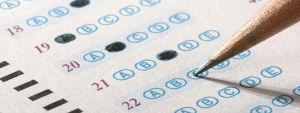
\includegraphics[width=3in]{scantron.png}
\end{figure}

In July 2016, the passing rate was $\approx$72\% of questions correct. For the purposes of this problem, assume this means 22 of the questions (or more) would have to be correct in order to pass. \\

We first consider the situation where the test-taker guesses the answer to each question by choosing one of the five equally likely choices. 

\benum
\subquestionwithpoints{3} Model the result of \emph{one} question below as a r.v. $X$ which has the value 1 if the answer is correct and 0 if the answer is not correct.  \spc{1}

\subquestionwithpoints{2} When guessing the answers to all 30 questions, are the r.v.'s that represent each question's correctness identically distributed? Yes / no. No explanation necessary.  \spc{0.2}

\subquestionwithpoints{2} When guessing the answers to all 30 questions, are the r.v.'s that represent each question's correctness independent? Yes / no. No explanation necessary.  \spc{0.2}

\subquestionwithpoints{3} Create a r.v. model that represents the total score for all 30 questions.  \spc{1}

\subquestionwithpoints{6} Compute the probability that the guesser gets \textit{exactly} 22 questions correct. Round to three significant digits.  \spc{4}

\subquestionwithpoints{3} If the guesser did the exam over and over again, what would his test average approximately be? \spc{1}

\subquestionwithpoints{6} Write an computable expression for the probability that the guesser passes the exam. Do not compute it explicitly.  \spc{3}

\subquestionwithpoints{5} Regardless of your answer in (g), do you think the guesser has a \textit{realistic} chance of passing? Yes / no and explain your answer. \spc{3}

\subquestionwithpoints{4} In the situtation where the test-taker knows something about some of the topics tested and uses that knowledge to answer some questions but guess on others which he has no knowledge of the topics, would the model built in (d) still be a good model for the test-taker's score on the exam? Yes / no and explain your answer. \spc{5}

\eenum


\problem Powerball is an American lottery game offered by 44 states, the District of Columbia, Puerto Rico and the US Virgin Islands. Since October 7, 2015, the game has used 5 white balls picked from 69 possible balls with replacement and onw \qu{powerball} with 26 possible balls resulting in a matrix from which winning numbers are chosen, resulting in odds of 1 in 292,201,338 of winning a jackpot per play (i.e. about three in a billion). Calculated as a probability, we denote the chance of winning as $p := 3.42 \times 10^{-9}$. \\

\begin{figure}[htp]
\centering
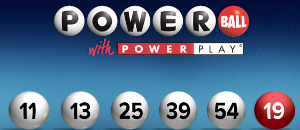
\includegraphics[width=3in]{powerball.png}
\end{figure}

Assume for simplicity that there is a powerball lottery every day, 365 days per year. Also assume when you buy a powerball lottery ticket, you pick a sequence of valid powerball numbers randomly (i.e. equally likely) for each ball.

\benum
\subquestionwithpoints{3} Create a r.v. $X$ for the outcome of one powerball lottery ticket which realizes 1 if you win and 0 if you lose. \spc{1}


\subquestionwithpoints{3} Consider the following strategy: buy a powerball ticket every day until you win. Create a r.v. model $X$ that models the number of days it takes to win. \spc{1}

\subquestionwithpoints{5} How many years would it take to win on average? Round to the nearest year. \spc{4}

\subquestionwithpoints{5} Imagine starting to play when you're 20 years old and stopping when you're 90 years old for a total of 70 years of daily playing. What is the probability of winning (at least once)? Round to two significant digits. \spc{5}


\subquestionwithpoints{5} Assuming you can play everyday \emph{forever}, what is the probability you eventually win? \spc{0.2}

\subquestionwithpoints{3} If you've been playing for 30 years without winning, do you have a higher chance of winning compared to someone who has just started playing? Yes / no. No explanation needed. \spc{0.2}

\subquestionwithpoints{5} Up until this point, we have just been discussing probabilities and modeling the event of winning or losing. Now we will put dollar amounts on these events. The powerball ticket costs \$2 and the average jackpot is \$140 million. Create a r.v. $X$ for the payout of \textit{one} powerball ticket. \spc{4}

\subquestionwithpoints{5} Calculate the expected value of $X$, (the r.v. model for the payout of \emph{one} powerball ticket in dollars). Round to an appropriate number of digits. \spc{5}

\subquestionwithpoints{5} Interpret the expected value you calculated in (i) in the scenario where you don't play for 70 years daily but you \textit{only play once}. \spc{4}

\subquestionwithpoints{6} Calculate the standard error of \emph{one} powerball lottery ticket.  Include units and round to an appropriate number of digits. \spc{8}


\subquestionwithpoints{4} Let's say you are buying the ticket in India where the currency is rupees (\rupee). The exchange rate is \$1 = \rupee66.80 and you have to pay a flat \rupee30 fee to purchase an American ticket from overseas. Create a r.v. $R$ for the lottery ticket bought in India with rupees as a function of the r.v. $X$ created in (h).\spc{2}

\eenum

\problem These are some theoretical questions below.

\benum
\subquestionwithpoints{3} If the r.v. $X \sim $ Deg($c$), prove $\expe{X} = c$ from the definition of expectation for discrete r.v.'s. \spc{5}

%\subquestionwithpoints{3} If $\Xoneton \iid$ with finite $\mu$ and $\sigma$, derive an expression for $\se{\Xbar}$ step-by-step. \spc{3}



\subquestionwithpoints{4} Compute the following expression for $w = 0.24586$:

\beqn
\sum_{\ell=y}^\infty \binom{\ell - 1}{y - 1} w^y (1-w)^{\ell - y}  = \quad\quad\quad\quad
\eeqn\spc{1}

\subquestionwithpoints{4} Assume $\expe{X_i} > 0$ and that $\Xoneton $ are \textit{identically distributed} but not necessarily independent. Resolve: \\

$\displaystyle\limitn \expe{T_n}  = $\spc{0.3}


\subquestionwithpoints{6} In your pocket you have 10 pennies, 2 nickels, 2 dimes and 3 quarters. You reach into your pocket and grab four coins in your hand. What's the probability you have 4\textcent~in your hand? \spc{15}


\subquestionwithpoints{4} [Extra Credit] Resolve the follwing expression for arbitrary r.v. $X$:

\beqn
\bigcup_{x \in \supp{X}} \braces{\omega : X(\omega) = x}  = \quad\quad\quad\quad
\eeqn

\subquestionwithpoints{4} [Extra Credit] Create a r.v. $X$ that has $\abss{\supp{X}} = 2$ but whose $\abss{\Omega} =  \aleph_0$.

\eenum


\end{document}